%# -*- coding: utf-8 -*-

\chapter{使用GDB}
\label{ch_gdb} \index{gdb}

\section{GDB简介}

GDB,全称\emph{The GNU Debugger},它能让你看到程序内部的执行过程,
程序如果通过~GDB~来启动话,还能修改程序执行过程,
GDB~还能用于检查程序异常退出产生的~core~文件。

GDB~支持如下四种启动方式,可以用于不同的目的。

\begin{enumerate}
\item 直接启动~GDB
\begin{lstlisting}
gdb
\end{lstlisting}
这种方式下,不需要任何参数,启动~GDB~后,会直接进入到~GDB~的提示符下。
通常要查看~GDB~的某些命令的帮助的时候可以这样做。
也可以使用这种方式启动~GDB~后,再使用~file~\index{gdb!file}命令载入可以执行文件进行调试,
使用~core~\index{gdb!file}命令来载入要调试的core文件。

\item \textbf{使用GDB启动一个待调试的程序}
\begin{lstlisting}
gdb program
\end{lstlisting}
这种方式启动的~GDB~需要跟一个参数~\param{program}~来指定要调试的可执行程序。
在使用~GDB~调试程序时候这种方式使用的比较多。如果要指定~\param{program}~的参数,
可以使用\shcmd{--args}\label{sec:gdb_args}参数,下面是一个示例:
\begin{lstlisting}
gdb -q --args foo -f foo.conf -x -p 19553
\end{lstlisting}
在\shcmd{--args}用于分隔~GDB~的参数和要调试的程序的参数,前面是~GDB~的参数,
后面的是要调试的程序及其运行的参数。
上面的命令含义是使用~GDB~的\shcmd{-q}参数来启动GDB,
要调试的程序是foo,foo的参数数"-f foo.conf -x -p 19553"。

\item \textbf{使用GDB调试一个正在执行的程序} \label{sec:gdb_start_attach}
\begin{lstlisting}
gdb program <pid>
\end{lstlisting}
\param{<pid>}是一个正在运行的程序\param{program}的进程号\footnote{如果存在一个名为<pid>的文件名,
GDB会把<pid>认为是一个core文件而载入这个core文件,而不是attach上进程号为<pid>的进程。},
以这种方式启动~GDB~后,GDB~会~attach~上该进程,
我们就可以对这个进程进行调试了。
比如我们调试后台运行的进程的就可以采用这种方式,
先由~daemon~进程把要调试的进程启动起来,然后我们再~attach~上去进行调试。

\item \textbf{使用GDB检查程序崩溃(crash)之后的core文件}
\begin{lstlisting}
gdb program core-file
\end{lstlisting}
这种方式启动~GDB~后,GDB~会从~\param{core-file}~读入程序\param{program}在crash时的内存映像。
通过~core~文件的信息,我们可以获知程序当是因为什么原因crash的。
关于调试~core~的更多信息参考第\ref{ch:coredump}章(第~\pageref{ch:coredump}~页)。

\end{enumerate}

% http://www.yolinux.com/TUTORIALS/GDB-Commands.html#GDB_COMMAND_LINE_ARGS

%%%%%%%%%%%%%%%%%%%%%%%%%%%%%%%%%%%%%%%%%%%%%%%%%%%%%%%%%%%%%%%%%%%%%%%
\section{GDB命令行参数}

GDB~支持的命令行参数简要介绍如下:

\noindent
--help\\
-h

显示~GDB~的帮助信息。

\noindent
--args

\paramdesc{用于分隔~GDB~的参数和它要调试的程序的参数,前面是~GDB~的参数,
后面的是要调试的程序及其运行的参数。参见~\pageref{sec:gdb_args}~页。}

\noindent
--exec=\param{file-name}\\
-e \param{file-name}

指定要调试的可执行文件名为\param{file-name}

\noindent
--core=\param{name-of-core-file}\\
-c \param{name-of-core-file}

指定要调试的~\code{core}~文件名~\param{name-of-core-file}。

\noindent
--command=\param{command-file}\\
-x \param{command-file}

\paramdesc{从文件~\param{command-file}~读入~GDB~命令并执行。
在命令文件中,使用‘\#’作为注释的起始符号。}

\noindent
--cd=\param{directory}

指定~GDB~运行时的\emph{当前工作目录}为~\param{directory}。

\noindent
--directory=\param{directory}\\
-d \param{directory}

添加目录~\param{directory}~到源代码的搜索路径中。

\noindent
--nx \\
-n

\paramdesc{忽略~GDB~的初始化脚本。启动时不执行~GDB~的初始化文件\$HOME/.gdbinit里的命令。}

\noindent
--quiet \\
-q

\paramdesc{安静模式。不显示介绍性的和版权信息。}

\noindent
--batch

\paramdesc{批处理模式,这个命令需要和~\underline{-x}~命令一起使用。
执行~\underline{-x}~指定的文件的命令,如果所有命令都执行成功,
gdb的退出值为0,否则退出值为非0。}

\noindent
--symbols=\param{file}\\
-s \param{file}

从\param{file}读入\emph{符号表(symbol table)}信息。


\noindent
-tui

\paramdesc{tui的全称是Text User Interface。启动基于文本模式的交互式界面。
它能在文本界面下模拟窗口显示源代码、汇编代码、寄存器信息和~GDB~的命令输出
(参见~\ref{sec:tui},第~\pageref{sec:tui}~页)。}

\noindent
-write

\paramdesc{允许对\emph{可执行文件}和\emph{core}文件进行写操作。
可以用于生成~patch。}

\noindent
-tty=\param{device}

指定设备\param{device}作为要调试程序的标志输入和输出。

\subsection{GDB命令示例}
\begin{lstlisting}
gdb -q foo
gdb -q foo 19553
gdb -q foo core-19553
gdb -q -x tmp.txt foo 19553
\end{lstlisting}

%%%%%%%%%%%%%%%%%%%%%%%%%%%%%%%%%%%%%%%%%%%%%%%%%%%%%%%%%%%%%%%%%%%%%%%

\section{GDB命令}

\subsection{获取帮助}
在~GDB~的命令提示符下可以使用~\code{help}~命令获取帮助信息。
不带参数的~\code{help}~命令会显示~GDB~命令类别的一个列表。如下所示:
\begin{lstlisting}
(gdb) help
List of classes of commands:

aliases -- Aliases of other commands
breakpoints -- Making program stop at certain points
data -- Examining data
files -- Specifying and examining files
internals -- Maintenance commands
obscure -- Obscure features
running -- Running the program
stack -- Examining the stack
status -- Status inquiries
support -- Support facilities
tracepoints -- Tracing of program execution without stopping the program
user-defined -- User-defined commands

Type "help" followed by a class name for a list of commands in that class.
Type "help all" for the list of all commands.
Type "help" followed by command name for full documentation.
Type "apropos word" to search for commands related to "word".
Command name abbreviations are allowed if unambiguous.
\end{lstlisting}
\code{help}~可以跟一个~GDB~的命令作为参数,会简要的描述一下这个命令的功能。
比如要查看~\code{watch}~命令的帮助信息,可以这样做:
\begin{lstlisting}
(gdb) help watch
Set a watchpoint for an expression.
A watchpoint stops execution of your program whenever
the value of an expression changes.
\end{lstlisting}

如果不知道确切的命令,可以使用\code{apropos}命令根据关键词\footnote{支持正则表达式。}来模糊查找~GDB~的所有命令和它的文档,
然后再使用~\code{help}~来获取相关命令的帮助信息。
比如要查找所有与~\code{core}~相关的信息,可以这样做:
\begin{lstlisting}
(gdb) apropos core
core-file -- Use FILE as core dump for examining memory
  and registers
gcore -- Save a core file with the current state of the
  debugged process
generate-core-file -- Save a core file with the current
  state of the debugged process
info files -- Names of targets and files being debugged
info line -- Core addresses of the code for a source line
info target -- Names of targets and files being debugged
maintenance -- Commands for use by GDB maintainers
maintenance dump-me -- Get fatal error; make debugger dump
  its core
maintenance info sections -- List the BFD sections of the
  exec and core files
maintenance set internal-error corefile -- Set whether
  GDB should create a core file of GDB when internal-error
  is detected
maintenance set internal-warning corefile -- Set whether
  GDB should create a core file of GDB when internal-warning
  is detected
maintenance show internal-error corefile -- Show whether
  GDB will create a core file of GDB when internal-error
  is detected
maintenance show internal-warning corefile -- Show whether
  GDB will create a core file of GDB when internal-warning
  is detected
mt -- Commands for use by GDB maintainers
set build-id-core-loads -- Set whether CORE-FILE loads
  the build-id associated files automatically
set write -- Set writing into executable and core files
show build-id-core-loads -- Show whether CORE-FILE loads
  the build-id associated files automatically
show write -- Show writing into executable and core files
target core -- Use a core file as a target
(gdb) help gcore
Save a core file with the current state of the debugged process.
Argument is optional filename.  Default filename is
  'core.<process_id>'.
\end{lstlisting}

在~\code{apropos}~列出的搜索结果中选择感兴趣的命令~\code{gcore},
然后在使用~\code{help}命令查看~\code{gcore}的帮助信息。

除此之外,还可以使用info命令(缩写为i)获取程序的状态,
你可以使用表~\ref{tab:gdb_help_info}~所列的info来获取程序的状态。
\begin{table}
\begin{tabularx}{400pt}{l|X}
\hline
\hline
GDB~命令 & 说明 \\
\hline
info frame      &   获取当前帧信息。\\
info stack      &   获取调用栈(同\code{bt})。\\
info args       &   获取当前帧的参数参数。\\
info locals     &   获取当前帧的局部变量信息。\\
info registers  &   获取当前寄存器的信息。\\
info threads    &   获取线程的信息。\\
info breakpoints    &   获取设置的断点信息。\\
info address $addr$   &   获取地址$addr$处的符号表信息。\\
info sharedlibrary  &   获取载入的动态库信息。\\
info symbol $addr$  &   获取$addr$处的符号表信息(只能获取全局的或静态范围的 TODO:refine desc)。\\
\hline
\hline
\end{tabularx}
\caption{使用info命令获取程序的状态信息}\label{tab:gdb_help_info}
\end{table}

使用info的示例如下:
\begin{lstlisting}
(gdb) info frame
Stack level 0, frame at 0xbffff6c0:
 eip = 0x8048c7e in foo (foo.cpp:24); saved eip 0x8048e50
 called by frame at 0xbffff700
 source language c++.
 Arglist at 0xbffff6b8, args: id=2, name=..., ctx=0xbffff6d4
 Locals at 0xbffff6b8, Previous frame's sp is 0xbffff6c0
 Saved registers:
  ebx at 0xbffff6b0, ebp at 0xbffff6b8, esi at 0xbffff6b4, eip at 0xbffff6bc
(gdb) info arg
id = 2
name = @0xbffff6d8
ctx = 0xbffff6d4
(gdb) info local
oss = <incomplete type>
key = {static npos = 4294967295,
  _M_dataplus = {<std::allocator<char>> = {<__gnu_cxx::new_allocator<char>> = {<No data fields>}, <No data fields>}, _M_p = 0x804c244 "2:SSA"}}
(gdb) info reg
eax            0xbffff6ac       -1073744212
ecx            0x0      0
edx            0x1      1
ebx            0x73aff4 7581684
esp            0xbffff5e0       0xbffff5e0
ebp            0xbffff6b8       0xbffff6b8
esi            0x0      0
edi            0x0      0
eip            0x8048c7e        0x8048c7e <foo(int, std::string const&, int**)+394>
eflags         0x282    [ SF IF ]
cs             0x73     115
ss             0x7b     123
ds             0x7b     123
es             0x7b     123
fs             0x0      0
gs             0x33     51
(gdb) info break
Num     Type           Disp Enb Address    What
1       breakpoint     keep y   0x08048aff in foo(int, std::string const&, int**) at foo.cpp:13
        breakpoint already hit 1 time
2       breakpoint     keep y   0x08048c7e in foo(int, std::string const&, int**) at foo.cpp:24
        breakpoint already hit 1 time
(gdb) info thread
* 1 process 12403  foo (id=2, name=..., ctx=0xbffff6d4) at foo.cpp:24
(gdb) info sharedlibrary
From        To          Syms Read   Shared Object Library
0x00d4f830  0x00d6569f  Yes         /lib/ld-linux.so.2
0x00eb7260  0x00f31088  Yes         /usr/lib/libstdc++.so.6
0x00d88460  0x00da2778  Yes         /lib/tls/i686/cmov/libm.so.6
0x00112370  0x0012a558  Yes         /lib/libgcc_s.so.1
0x00610930  0x00704eac  Yes         /lib/tls/i686/cmov/libc.so.6
(gdb) info symbol 0x8048aff
foo(int, std::string const&, int**) + 11 in section .text of /home/chenming/sandbox/a.out
(gdb) info stack
#0  foo (id=2, name=..., ctx=0xbffff6d4) at foo.cpp:24
#1  0x08048e50 in main () at foo.cpp:46
\end{lstlisting}

更多的关于~\code{info}~的信息可以通过~\code{help info}~来获得。

\subsection{Shell命令}
在~GDB~的命令提示符下可以执行~\shcmd{shell}~的命令,可以使用
\begin{lstlisting}
shell command string
\end{lstlisting}
来执行\shcmd{shell}命令。比如:
\begin{lstlisting}
shell ls -lrt /var/crash/
\end{lstlisting}

GDB~内建的~\shcmd{make}~命令可以直接使用,
这在调试程序时修改代码后要立即编译的时候非常有用。\shcmd{make}命令的语义如下:
\begin{lstlisting}
make make-args
\end{lstlisting}
它等价于:
\begin{lstlisting}
shell make make-args
\end{lstlisting}

\subsection{记录GDB的输出}
如果想记录在调试过程中~GDB~的输出到指定的文件,可以使用表~\ref{tab:gdb_logging}~中的命令。
这些命令可以用来控制~GDB~的输出。

\begin{table}[!bhp]
\begin{tabularx}{400pt}{l|X}
\hline
\hline
命令 & 说明 \\
\hline
set logging on                  &   开启日志功能。  \\
set logging off                 &   关闭日志功能。  \\
set logging file $filename$     &   改变当前日志文件名称,缺省的日志文件名为'gdb.txt'。 \\
set logging overwrite [on|off]  &   缺省情况下,GDB~会以追加的方式写日志文件,
                                    如果这个参数为on,那么~GDB~会以覆盖的方式写日志文件。\\
set logging redirect [on|off]   &   缺省情况下,GDB~会在屏幕上和日志文件中都写入命令的输出,
                                    如果这个参数为on,那么~GDB~只会把命令输出写入日志文件。\\
show logging                    &   显示当前日志的设置情况。\\
\hline
\hline
\end{tabularx}
\caption{GDB的logging相关命令} \label{tab:gdb_logging}
\end{table}

下面是一个设置logging的实例:
\begin{lstlisting}
(gdb) set logging file gdb.log
(gdb) set logging on
Copying output to gdb.log.
(gdb) show logging
Currently logging to "gdb.log".
Logs will be appended to the log file.
Output will be logged and displayed.
(gdb) q
\end{lstlisting}

\subsection{命令输入}
GDB~支持\emph{命令补全}\index{gdb!命令补全},
使用Tab键可以补全命令,这个功能与shell的命令补全功能类似,
如果有多个备选项,连续按两次Tab键可以显示所有的备选项。

GDB~还支持\emph{命令缩写}\index{gdb!命令缩写},即指输入命令的前几个字符,
如果这几个字符就可以把它和其它的命令区分开了的话,
就能使用这种命令缩写,比如info reg就是info register的缩写。

在~GDB~的命令提示符下,如果不输入命令而直接按回车,
它的含义是重复上一条命令,但对于一些特殊的命令,比如run命令,它不会重复。
对于list和x命令的重复,GDB~会根据上下文来决定新的命令参数以便于我们连续的浏览代码和内存信息。

在~GDB~中使用~\#~作为\emph{注释}的起始符,任何~\#~后面的内容都会被~GDB~忽略。
它主要用于命令文件中。

在~GDB~的命令提示符下,还支持表~\ref{tab:gdb_shortcut}~中的快捷键来快速的浏览、编辑和查找历史命令。

\begin{table}[!bhp]
\begin{tabularx}{400pt}{l|X}
\hline
\hline
快捷键  &   说明    \\
\hline
Ctrl+n  &   下一条命令  \\
Ctrl+p  &   上一条命令  \\
Ctrl+r  &   反向搜索    \\
Ctrl+l  &   清屏        \\
Ctrl+a  &   跳到行首    \\
Ctrl+e  &   跳到行尾    \\
Ctrl+b  &   向左移动光标    \\
Ctrl+f  &   向右移动光标    \\
Ctrl+k  &   删除到行尾      \\
Ctrl+u  &   删除到行首(很常用吧)      \\
Ctrl+d  &   删除当前光标所在的字符    \\
\hline
\hline
\end{tabularx}
\caption{GDB命令提示符下可用的快捷键} \label{tab:gdb_shortcut}
\end{table}


\section{在GDB控制下运行程序}
\subsection{影响调试的GCC选项}
为了能够使用~GDB~方便的调试程序,
需要在使用~GCC~编译程序的时候生成调试信息。
最常用的生成调试信息的编译选项为~\code{-g}。
如果要包含\emph{宏}相关的信息,需要使用“\code{-gdwarf-2 -g3}”,
\code{-gdwarf-2}~指定调试信息的格式为Dwarf-2,
\code{-g3}会产生更多额外的调试信息。

如果在编译时指定优化选项(\code{-O、-O1、-O2~或~-O3}),
经过编译器优化后,产生的代码的执行顺序可能会与源代码中不一致,
这会导致调试时侯很不方便,因此建议在调试程序的时候不要做任何优化。

在编译调试版本的时候如果使用~\code{-fno-inline}参数也会帮助我们调试,
它会去掉内联优化。

表~\ref{tab:gdb_gcc_opt}~列出了~GCC~编译时会影响调试的选项。

\begin{table}[!bhp]
\begin{tabular}{l|l}
\hline
\hline
选项 & 说明 \\
\hline
-g		&   带上调试信息        \\
-g  3   &   带上更多的调试信息  \\
-O0		&   去掉优化            \\
-fstack-check	&   增加栈溢出的检查    \\
-fno-inline     &   去掉inline优化      \\
-fomit-frame-pointer    &   优化掉帧指针,要调试程序时不要使用这个选项 \\
\hline
\hline
\end{tabular}
\caption{影响调试的GCC选项} \label{tab:gdb_gcc_opt}
\end{table}

调试程序建议的编译选项为:
\begin{lstlisting}
-g -fno-inline -O0
\end{lstlisting}
或:
\begin{lstlisting}
-gdwarf-2 -g3 -fno-inline -O0
\end{lstlisting}

\subsection{启动被调试的程序}
使用命令~\code{run}~(缩写为~\code{r})可以在~GDB~下开始运行要调试的程序。
如果要调试的程序需要命令行参数,直接跟在\code{run}命令后面就是了。示例:
\begin{lstlisting}
(gdb) r -p 19553
Starting program: /home/cm/sandbox/a.out -p 19553
\end{lstlisting}

在~\code{run}中指定参数的一个缺点就是每次执行程序的时候都需要指定一次,
比较麻烦。
另一种指定程序参数的方法是使用~\code{set args}~命令,设置好参数后,
以后执行简单的执行~\code{run}~命令就可以使用之前设置好的参数来启动程序了。
示例:
\begin{lstlisting}
(gdb) set args -p 19553
(gdb) r
Starting program: /home/cm/sandbox/a.out -p 19553
\end{lstlisting}

在调试程序的时候可以使用~\code{show args}~来查看程序的启动参数。示例:
\begin{lstlisting}
(gdb) show args
Argument list to give program being debugged when it is started is "-p 19553".
\end{lstlisting}

要结束当前正在调试的进程,可以使用~\code{kill}命令:
\begin{lstlisting}
(gdb) kill
\end{lstlisting}

\subsection{调试正在运行的程序}
如果一个程序已经运行了,
比如这个程序是一个后台服务进程或者这个进程是由其它进程启动的子进程。
我们想要调试它,
可以使用第~\ref{sec:gdb_start_attach}~节(第~\pageref{sec:gdb_start_attach}~页)给出的方法。
另外一种调试正在运行的程序的方法就是使用~\code{attach}~命令。
\code{attach}~命令需要一个参数~\param{pid}~用来指定正在运行的程序。

在结束调试后,需要使用~\code{detach}~命令来释放~GDB~对正在调试程序的控制权。
如果在退出~GDB~前没有使用~\code{detach}~命令,
GDB~会提示你是否~\code{detach},
如果你选择了''\emph{否}'',gdb会杀掉正在调试的程序。

示例
\begin{lstlisting}
gdb httpd
(gdb) attach 19553
(gdb) b file:line
(gdb) c
...
(gdb) detach
\end{lstlisting}

\subsection{调试子进程} \index{gdb!调试子进程}

通常使用~GDB~调试子进程的方式是在子进程里插入\code{sleep()}语句。
运行~GDB~进行调试这个程序,等到子进程被\code{fork}后,
得到它的进程号,然后在另外一个终端运行~GDB,
用这个进程号~\code{attach}~上这个子进程,我们就可以调试子进程了。

另外一种方式是在~GDB~中设置~\code{follow-fork-mode}
\index{gdb!follow-fork-mode}为\code{child},
它的使用方式是~\code{set follow-fork-mode child}。
缺省~GDB~会跟踪父进程。

可以使用~\code{show follow-fork-mode}~查看当前的设置:
\begin{lstlisting}
(gdb) show follow-fork-mode
Debugger response to a program call of
  fork or vfork is "parent".
(gdb) set follow-fork-mode child
(gdb) show follow-fork-mode
Debugger response to a program call of
  fork or vfork is "child".
\end{lstlisting}

\subsection{调试多线程程序}
如果要调试的程序是多线程的,可以使用~\code{info threads}~来查看当前所有线程的信息。
示例:
\begin{lstlisting}
%TODO:
\end{lstlisting}

\code{info threads}~会输出每个线程的线程号,
接下来可以使用~\code{thread $n$}~来切换到该线程,其中$n$是要切换到的线程号。
切换到该线程后就可以对这个线程进行调试了。
示例:
\begin{lstlisting}
(gdb) thread n
%TODO:
(gdb) bt
..
\end{lstlisting}

在有多个线程的时候,如果想对每个线程都执行相同的命令,
比如想执行~\code{bt}~命令检查每个线程的调用栈,可以使用命令
\code{thread apply all $args$},$args$是要执行的命令。示例:
\begin{lstlisting}
thread apply all bt
\end{lstlisting}
这条命令就会显示当前所有线程的调用栈。
调试多线程的时候,这条命令被经常使用。

\section{跟踪程序执行}
使用调试器的一大方便点就是在于它能够跟踪程序的执行过程,
这一节的主要内容包括如何设置程序断点、如何处理信号以及单步跟踪程序的执行。

要知道被调试的程序是否正在运行,以及运行的状态,
可以在调试器中可以使用~\code{info program}~查看当前调试程序的状态。示例:
\begin{lstlisting}
(gdb) info program
   Using the running image of child process 14058.
Program stopped at 0x8048aff.
It stopped at breakpoint 1.
\end{lstlisting}

\subsection{断点的设置}
GDB~的\emph{断点}包括三种:
\begin{description}
\item[breakpoint] \index{gdb!breakpoint}是最常用的断点类型,
可以使用\emph{行号}(格式为\code{file:lineno}),
\emph{函数名}(C++如果有名字空间,需要在函数名前加名字空间)
或\emph{地址}来指点\emph{breakpoint}。
在指定~\emph{breakpoint}~的时候还可以附加条件。
对于位于动态库中的断点,
GDB~支持在未加载的动态库的时候先设置\emph{breakpoint}\footnote{
对这种情况GDB会给出类似这样的提示:
"Make breakpoint pending on future shared library load? (y or [n])"。},
这种类型的断点称之为\code{pending breakpoint}。
如果要设置动态库的\emph{breakpoint},建议使用\emph{行号}的方式来指定。
如何设置\emph{breakpoint}参见第~\pageref{sec:gdb_breakpoint}~页。

\item[watchpoint] \index{gdb!watchpoint}是一种特殊的断点,
只有当watch的表达式的值改变时程序才会中断。
如何设置\emph{watchpoint}参见第~\pageref{sec:gdb_watchpoint}~页。

\item[catchpoint] \index{gdb!catchpoint}也是一种特殊的断点,
它能捕获特殊的事件,比如C++的异常,加载一个动态库等。
如何设置\emph{catchpoint}参见第~\pageref{sec:gdb_catchpoint}~页。
\end{description}

GDB~使用数字来标识已经设置了断点,第一个设置断点编号为1,第二个为2,以此类推\ldots
在删除和临时禁止断点的时候需要使用这些编号。

\subsubsection{breakpoint的设置}
\label{sec:gdb_breakpoint} \index{gdb!breakpoint}
使用~\emph{breakpoint}~的命令的为~\code{break}(缩写为~\code{b})。
GDB~的内置变量\code{\$bpnum}记录了你最近设置的~\emph{breakpoint}~的编号。
可以使用如下几种方式设置断点:

\noindent
\code{break \param{func}}

\paramdesc{参数~\param{func}~是\emph{函数名}。
这种方式在函数的入口点设置~\emph{breakpoint}。}

\noindent
\code{break \param{lineno}}

\paramdesc{参数~\param{lineno}~是\emph{行号}。
这种方式在当前源文件的指定行设置~\emph{breakpoint}。}

\noindent
\code{break \param{filename:lineno}}

\paramdesc{参数~\param{filename:lineno}~是\emph{文件名:行号}。
这种方式在指定的源文件的指定行号处设置~\emph{breakpoint}。}

\noindent
\code{break *\param{addr}}

\paramdesc{参数~\param{addr}~是\emph{指令的地址}。
在没有调试信息情况下可以使用这种方式设置~\emph{breakpoint}。}

\noindent
\code{break}

\paramdesc{对于没有参数的~\code{break}~命令,会在下一条指令处设置~\emph{breakpoint}。}

\noindent
\code{break \param{args} if \param{cond}}

\paramdesc{带~\code{if}~的~\code{break}~命令可以用于设置条件断点\index{gdb!条件断点},
参数\param{cond}是用来设置中断的条件,只有当条件满足时程序才会中断。
\param{args}~是要前面描述的\code{break}可以使用的参数。
一个设置条件断点的实例:\code{break bar if i < 0}。}

\noindent
\code{tbreak \param{args}} \index{gdb!tbreak}

\paramdesc{设置\emph{一次性断点}。
\param{args}~与~\code{break}~命令的参数一致,
设置方法也与~\code{break}~命令一致。
与\code{break}设置的永久性断点不同,
\code{tbreak}设置的断点在程序第一次中断之后会自动删除。}

\noindent
\code{hbreak \param{args}} \index{gdb!hbreak}

\paramdesc{设置\emph{硬件断点}。\param{args}~与~\code{break}~命令的参数一致。
\emph{硬件断点}需要硬件的支持,一般来说硬件断点会有个数的限制。}

\noindent
\code{thbreak \param{args}} \index{gdb!thbreak}

设置\emph{一次性的硬件断点}。

\noindent
\code{info breakpoints [\param{n}]}\\
\code{info break [\param{n}]}\\
\code{info watchpoints [\param{n}]}

\paramdesc{显示系统已经设置了的~\emph{breakpoints}、\emph{watchpoints}、
和~\emph{catchpoints}~列表。
如果带参数~\param{n}~的话会只显示第~\param{n}~个断点的信息。}

GDB~内部也会设置一些断点用于特殊的目的,
比如用于正确的处理~\code{longjmp},
这类断点的编号都是负数,而且使用~\code{info breakpoints}是看不到的。
要查看这类断点,需要使用命令~\code{maint info breakpoints}。
\index{gdb!maint info breakpoints}

设置~\emph{breakpoint}~的示例:
\begin{lstlisting}
(gdb) b main
Breakpoint 1 at 0x80483f3: file foo.c, line 10.
(gdb) b foo.c:12
Breakpoint 2 at 0x8048404: file foo.c, line 12.
(gdb) tbreak  bar
Breakpoint 3 at 0x80483ba: file foo.c, line 4.
(gdb) info break
Num Type       Disp Enb Address    What
1   breakpoint keep y   0x080483f3 in main at foo.c:10
    breakpoint already hit 1 time
2   breakpoint keep y   0x08048404 in main at foo.c:12
3   breakpoint del  y   0x080483ba in bar at foo.c:4
(gdb) main info breakpoints
Num Type       Disp Enb Address    What
-1  longjmp resume keep n   0x00000000
1   breakpoint keep y   0x080483f3 in main at foo.c:10
2   breakpoint keep y   0x08048404 in main at foo.c:12
3   breakpoint del  y   0x080483ba in bar at foo.c:4
\end{lstlisting}

\subsubsection{watchpoint的设置}
\label{sec:gdb_watchpoint} \index{gdb!watchpoint}
\emph{watchpoint}~会在监视的表达式的值改变的时候中断程序的执行,
用于跟踪变量的改变非常有用,它能准确的找出变量发生改变的地方。

根据系统的不同,\emph{watchpoint}~的实现可以是软件或硬件的,
如果是软件的实现,GDB~会单步执行程序并且检查监视的表达式是否发生改变,
这样会导致程序的执行效率成百倍的降低。
而在支持硬件~\emph{watchpoint}~的系统如~HP-UX、基于x86的CPU的系统,
GDB会使用硬件~\emph{watchpoint},这不会导致执行效率的降低。

设置~\emph{watchpoint}~的命令如下:

\noindent
\code{watch \param{expr}} \index{gdb!watch}

\paramdesc{设置一个~\emph{watchpoint}~用来监视表达式~\param{expr}的改变,
当~\param{expr}~的值发生改变的时候,中断程序的执行。}


\noindent
\code{rwatch \param{expr}} \index{gdb!rwatch}

\paramdesc{设置一个~\emph{watchpoint}~用来监视对表达式~\param{expr}的读取动作,当~\param{expr}~的被读取的时候,中断程序的执行。}

\noindent
\code{awatch \param{expr}} \index{gdb!awatch}

\paramdesc{设置一个~\emph{watchpoint}~用来监视对表达式~\param{expr}的读取或改变的动作,
当~\param{expr}~的被读取或改变的的时候,中断程序的执行。}

\code{rwatch}~和~\code{awatch}~只能在使用实现了硬件~\emph{watchpoint}的平台上使用。

如果是设置局部变量的~\emph{watchpoint},需要程序运行到相应的函数里才能进行设置。

设置~\emph{watchpoint}~的示例:
\begin{lstlisting}
(gdb) watch buf
Hardware watchpoint 2: buf
(gdb) info watchpoints
Num Type          Disp Enb Address    What
1   breakpoint    keep y   0x080483ba in bar at foo.c:4
    breakpoint already hit 1 time
2   hw watchpoint keep y              buf
\end{lstlisting}

\subsubsection{catchpoint的设置}
\label{sec:gdb_catchpoint} \index{gdb!catchpoint}

\emph{catchpoint}~能用于捕捉一些特殊的事件,比如C++的异常、系统调用、fork等。
使用命令~\code{catch}~来设置~\emph{catchpoint}。

\noindent
\code{catch \param{event}} \index{gdb!catch}

\paramdesc{在指定的事件~\param{event}~上中断程序的执行。
\param{event}见表~\ref{tab:catch_event}。}

\noindent
\code{tcatch \param{event}} \index{gdb!tcatch}

\paramdesc{在指定的事件~\param{event}~上设置一次性的\emph{catchpoint}。}


\begin{table}[!bhp]
\begin{tabularx}{400pt}{l|X}
\hline
\hline
事件名称 & 描述 \\
\hline
\code{throw} & C++异常的throw。\\
\code{catch} & C++异常的catch。\\
\code{exec}  & exec()调用。\\
\code{fork}  & fork()调用。\\
\code{vfork} & vfork()调用。\\
\code{syscall [\param{name}]}
             & 系统调用,\param{name}~为系统调用的名字,
               如果没有指定,会~catch~所有的系统调用。\\
\hline
\hline
\end{tabularx}
\caption{catch支持的事件类型}\label{tab:catch_event}
\end{table}

设置了~\emph{catchpoint}~之后,可以使用~\code{info breakpoints}~命令查看。

\textbf{对C++异常的调试}:
有时程序中有未捕获的异常会导致程序异常的行为甚至导致程序的直接退出。
这对服务器程序来说是不可接受的。这个时候我们可以使用GDB的\code{catch
throw}来捕获异常,设置这样的\emph{catchpoint}之后,如果再产生异常的话,
GDB就会中断程序的执行,
我们就可以使用~GDB~的\emph{bt}命令来检查出现错误的调用栈了。

\code{catch}~不支持对\emph{信号}的捕获,如果要捕获信号,
需要使用\code{handle}命令,
参见第~\ref{sec:gdb_handle}~节(第~\pageref{sec:gdb_handle}~页)。

设置~\emph{catchpoint}~的示例:
\begin{lstlisting}
(gdb) catch throw
Catchpoint 1 (throw)
(gdb) catch fork
Catchpoint 2 (fork)
(gdb) cat syscall clone
Catchpoint 3 (syscall 'clone' [120])
(gdb) info breakpoints
Num Type       Disp Enb Address    What
1   breakpoint keep y   0x081abd84 exception throw
2   catchpoint keep y              fork
3   catchpoint keep y              syscall "cl
\end{lstlisting}

\subsection{断点的删除}
删除断点可以使用~\code{clear}~\index{gdb!clear}或~\code{delete}~\index{gdb!delete}命令。\code{clear}~命令用于删除指定位置的代码,\code{delete}~需要使用之前设置的断点的编号作为参数。

\noindent
\code{clear [\param{location}]}

\paramdesc{不带参数的clear命令会删除所有已经设置的断点。
参数\param{location}~可以用于指定要删除的断点的具体位置,
\param{location}~可以使用函数名、行号、文件名:行号等几种格式。}

\noindent
\code{delete [breakpoints] [\param{range...}]}

\paramdesc{不带参数的~\code{delete}~命令
(缩写为~\code{d})会删除所有已设置的断点。
参数~\param{range}~用于指定要删除的断点范围,
可以是一个断点,也可以是多个断点,多个断点之间使用空格分隔,
如果断点的范围是连续的,还可以使用减号指定范围。
可以使用~\code{info breakpoints}~来查看已经设置了断点列表。}

删除断点的示例:
\begin{lstlisting}
(gdb) delete breakpoints 3
(gdb) delete breakpoints 2 3 5
(gdb) delete breakpoints 2-5
(gdb) delete breakpoints 1 2-5
\end{lstlisting}

\subsection{禁止/启用断点}
\index{gdb!禁止断点}

使用~\code{clear}~或~\code{delete}~删除\emph{断点},
会让这个断点彻底的消失,
一般情况下我们只是想临时的禁止这个断点,之后在重新启用。
GDB~的~\code{disable}(缩写为~\code{dis})~和~\code{enable}~命令提供这种功能。

\noindent
\code{disable [breakpoints] [\param{range\ldots}]}

\paramdesc{如果没有参数,会禁止所有的断点。
参数~\param{range}~是断点的编号,可以指定要禁用的断点的范围。}

\noindent
\code{enable [breakpoints] [\param{range\ldots}]}

\paramdesc{如果没有参数,会重新启用所有的断点。
参数~\param{range}~是断点的编号,可以指定要启用的断点的范围。}

\noindent
\code{enable [breakpoints] once \param{range\ldots}}

\paramdesc{临时性的启用断点。在这个断点被中断一次之后立即禁用。}

\noindent
\code{enable [breakpoints] delete \param{range\ldots}}

\paramdesc{一次性的启用断点。在这个断点被中断一次之后立即删除该断点。
使用~\code{tbreak}~设置的断点就是这种类型。}

禁用/启用了断点之后可以使用~\code{info break}~查看断点的状态。

禁用和启用断点的示例:
\begin{lstlisting}
(gdb) disable breakpoints 2
(gdb) disable breakpoints 3 5-7
(gdb) enable 2
(gdb) enable breakpoints once 2
(gdb) enable once 2
(gdb) enable delete 5
\end{lstlisting}

\subsection{断点命令列表}
在设置断点(\emph{breakpoint、watchpoint、catchpoint})时候可以指定一系列的命令在程序该断点中断的时候执行,
比如你可以在这些命令中打印一些变量的值,启用或禁用其它的断点等。

断点命令列表如下:

\noindent
\code{commands [\param{bnum}]   \\
\ldots \param{command-list} \ldots  \\
end}

\paramdesc{\param{bnum}~指定在该编号的断点被中断的时候执行相应的命令序列。
如果没有指定~\param{bnum},那么~\code{commands}针对最近的一个断点设置命令。
命令列表可以分多行,以~\code{end}~作为命令列表的结束。
如命令列表的第一个命令是~\code{silent}~,那么~GDB~不会打印在该断点上中断的信息。
\code{silent}~主要用在你只想在某些点检查一些变量的值而不想中断程序的执行的时候非常有用。
你可以使用~\code{echo}、\code{output}~和~\code{printf}~来精确的控制命令的输出格式。比如,下面的命令会在~\code{x > 0}~的时候打印函数~\code{foo}~参数及~\code{x}~的值,
因为使用了~\code{continue}~的原因,在打印了我们需要的信息之后程序会继续执行:}
\begin{lstlisting}
break foo if x > 0
commands
silent
info args
printf "x is %d\n", x
continue
end
\end{lstlisting}

\subsection{继续执行和单步执行}
\emph{继续执行}会继续程序的执行,直到下一个断点或者程序结束,
\emph{继续执行}在~GDB~中的对应的命令为~\code{continue}(缩写为~\code{c})。
\emph{单步执行}可以一条机器指令或一行源代码。
\emph{单步执行}对应的~GDB~命令有\code{next}、\code{step}等。

\noindent
\code{continue [\param{ignore-count}]}

\paramdesc{\emph{继续执行}。
可选参数~\param{ignore-count}~可以用于指定在继续执行之后忽略当前断点次数。}

\noindent
\code{step [\param{count}]}

\paramdesc{\emph{单步执行(步入)}。命令缩写为~\code{s}。
如果没有参数,执行一行源代码,如果遇到函数会进入到函数里面
可选参数~\param{count}~用于指定要单步执行的步数,
如果在~\param{count}~之前遇到断点,会提前中断。}

\noindent
\code{next [\param{count}]}

\paramdesc{\emph{单步执行}。命令缩写为~\code{n}。
如果没有参数,执行一行源代码,如果遇到函数不进入到函数里面
(如果要进行函数,需要使用~\code{step}~命令)。
可选参数~\param{count}~用于指定要单步执行的步数,
如果在~\param{count}~之前遇到断点,会提前中断。}

\noindent
\code{stepi [\param{count}]}

\paramdesc{\emph{单步执行一条机器指令(步入)}。命令缩写为~\code{si}。
配合~\code{display/i \$pc}~使用效果比较好。
可选参数~\param{count}同命令~\code{step}~的参数。}


\noindent
\code{nexti [\param{arg}]}
\paramdesc{\emph{单步执行一条机器指令}。命令缩写为~\code{ni}。
如果是函数调用,不进入到函数内部。
可选参数~\param{count}同命令~\code{next}~的参数。}

\noindent
\code{finish}
\label{sec:cmd_finish}

\paramdesc{\emph{执行完当前函数并返回}。命令缩写为~\code{fin}。
如果不想继续执行当前函数剩下的代码而直接返回,
需要使用~\code{return}~命令
(参见第~\ref{sec:cmd_return}~节,第~\pageref{sec:cmd_return}~页)。}


\subsection{处理信号}
\label{sec:gdb_handle}
\index{gdb!调试信号}

在~GDB~中可以使用~\code{handle}~命令来捕获和处理信号,
在收到指定的信号时中断程序的执行。

\noindent
\code{handle \param{signum} [\param{actions}\ldots]}

\paramdesc{参数~\param{signum}~是要处理的信号,
它可以是信号名,比如~\code{SIGSEGV}(也可以写成~\code{SEGV},
不要~\code{SIG}前缀),
也可以是数字格式,比如~11。
如果要指定所有的信号,可以使用关键字'\code{all}',
它代表所有已知的信号。\\
参数~\param{actions}~用来指定~GDB~在收到指定信号后的动作。
它可以是表~\ref{tab:signal_actions}~中的值。
可以同时指定多个动作。}

\begin{table}[!bhp]
\begin{tabularx}{400pt}{l|X}
\hline
\hline
action	& 说明 \\
\hline
nostop  & 收到该信号时不中断程序执行。\\
stop    & 收到该信号时中断程序执行。\\
print   & 收到该信号时打印信息。\\
noprint & 收到该信号时不打印信息。\\
pass    & 传递该信号给被调试的程序,由被调试的程序处理该信号。\\
nopass  & 不传递该信号给被调试的程序。\\
\hline
\hline
\end{tabularx}
\caption{handle支持的action} \label{tab:signal_actions}
\end{table}

在~GDB~中,程序被信号中断执行时,信号还没有被传递给被调试的程序,
直到你使用~\code{continue}~继续程序执行执行被调试程序才会收到信号。

如果是~GDB 7.0~,
GDB~内置了一个变量~\code{\$\_siginfo}~用于记录产生的信号的信息。
一般来说~\code{\$\_siginfo}~的类型为~\code{siginfo\_t},
在~\code{signal.h}~中有定义。
可以使用~\code{ptype \$\_siginfo}来检查,参见本节示例。

在~GDB~中可以使用~\code{info handle}~来查看信号的行为。

\noindent
\code{info handle \param{signum}}

\paramdesc{查看信号~\param{signum}~当前收到信号的行为。
如果没有指定参数~\param{signum},默认会显示所有的信号行为。}

在~GDB~中处理信号的示例:
\begin{lstlisting}
(gdb) handle SIGPIPE
Signal  Stop Print Pass to program  Description
SIGPIPE No   Yes   Yes              Broken pipe

(gdb) handle SIGUSR1 nostop print
Signal  Stop Print Pass to program  Description
SIGUSR1 No   Yes   Yes		    User defined signal 1

(gdb) info handle SIGPIPE
Signal  Stop Print Pass to program  Description
SIGPIPE No   Yes   Yes              Broken pipe

(gdb) info handle SIGSEGV
Signal  Stop Print Pass to program  Description
SIGSEGV Yes  Yes   Yes              Segmentation fault
\end{lstlisting}

使用~\code{\$\_signinfo}~的例子,
在这个例子中因为收到~\code{SIGSEGV}~信号中断了程序的执行,
通过打印~\code{\$\_signinfo}~来检查非法的内存访问点。
\begin{lstlisting}
(gdb) c
Continuing.

Program received signal SIGSEGV, Segmentation fault.
0x0804b5da in main () at foo.cpp:97
97	    *p = 0;
(gdb) p $_siginfo._sifields._sigfault
$4 = {
  si_addr = 0xb5bff4
}
\end{lstlisting}

\section{检查堆栈}
\index{gdb!栈} \index{gdb!stack}
\index{gdb!帧} \index{gdb!frame}

\emph{栈}(\emph{stack})是程序在执行函数调用时用来保存当前状态和传递参数的。
\emph{栈}由\emph{帧}(\emph{frame})组成,每次函数调用就形成一个新的~\emph{帧}。

\subsection{栈(stack)}
栈的结构如图~\ref{fig:stack_frame}~所示\footnote{该图来自~GDB~源代码包。位置为~gdb/doc/stack\_frame.eps}。

\begin{figure}
\begin{center}
% 缩放到文本宽度的90%
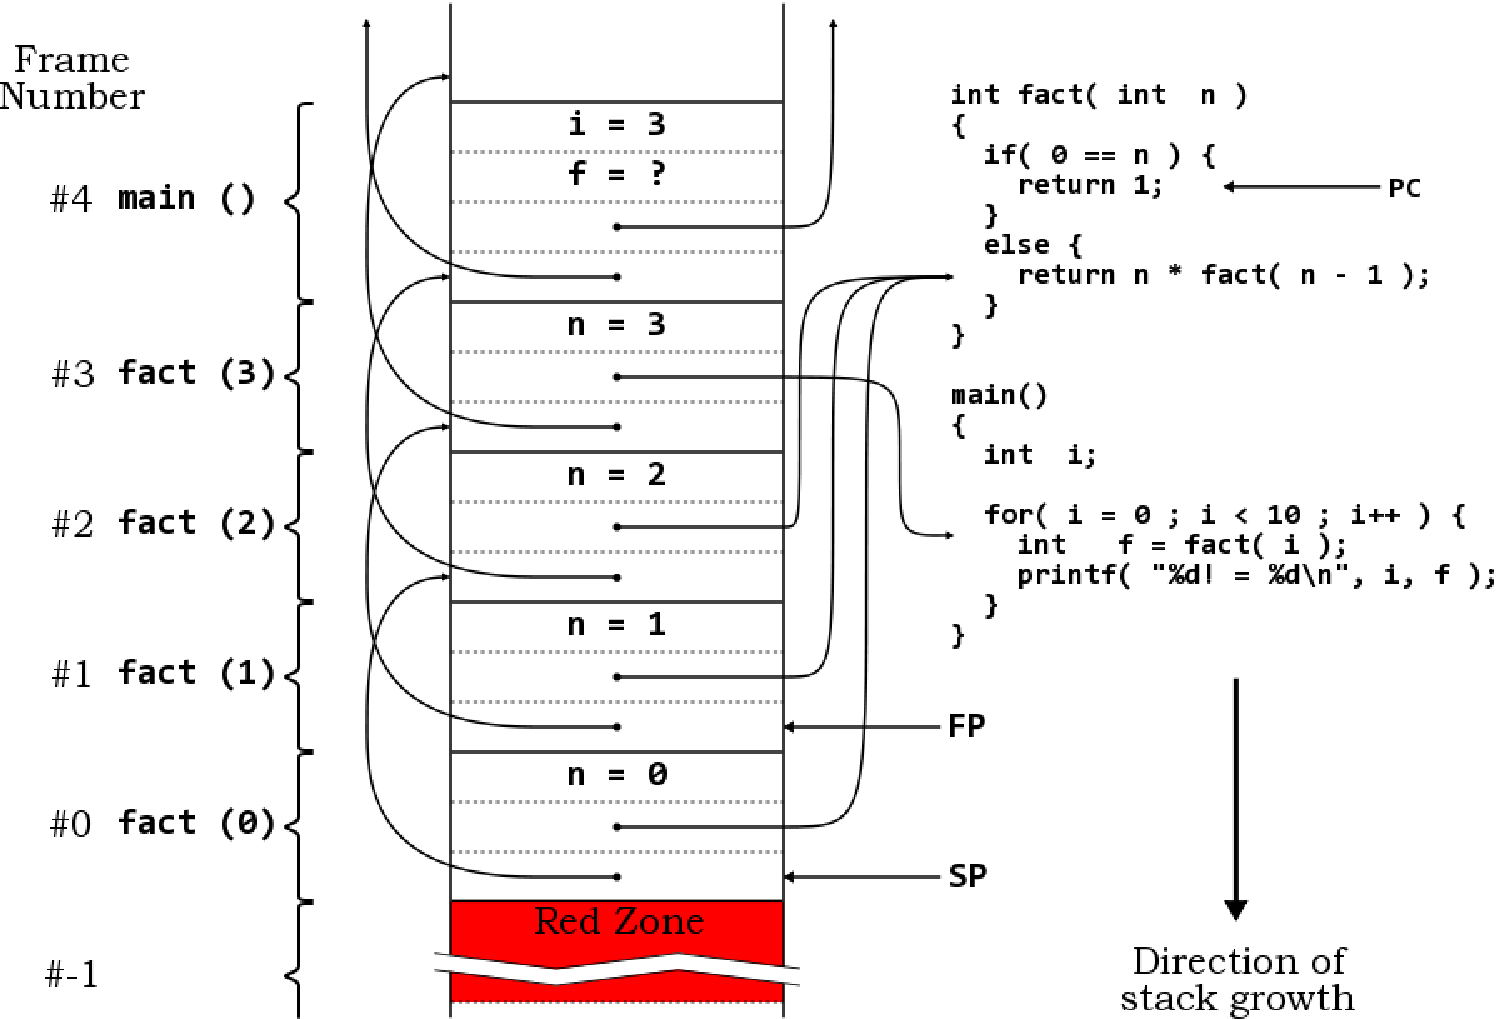
\includegraphics[width=0.9\textwidth]{figure/stack_frame}
\caption{栈和帧} \label{fig:stack_frame}
\end{center}
\end{figure}

图~\ref{fig:stack}~是一个更详细的描述栈和帧的图。
\begin{figure}
\begin{center}
% 缩放到文本宽度的90%
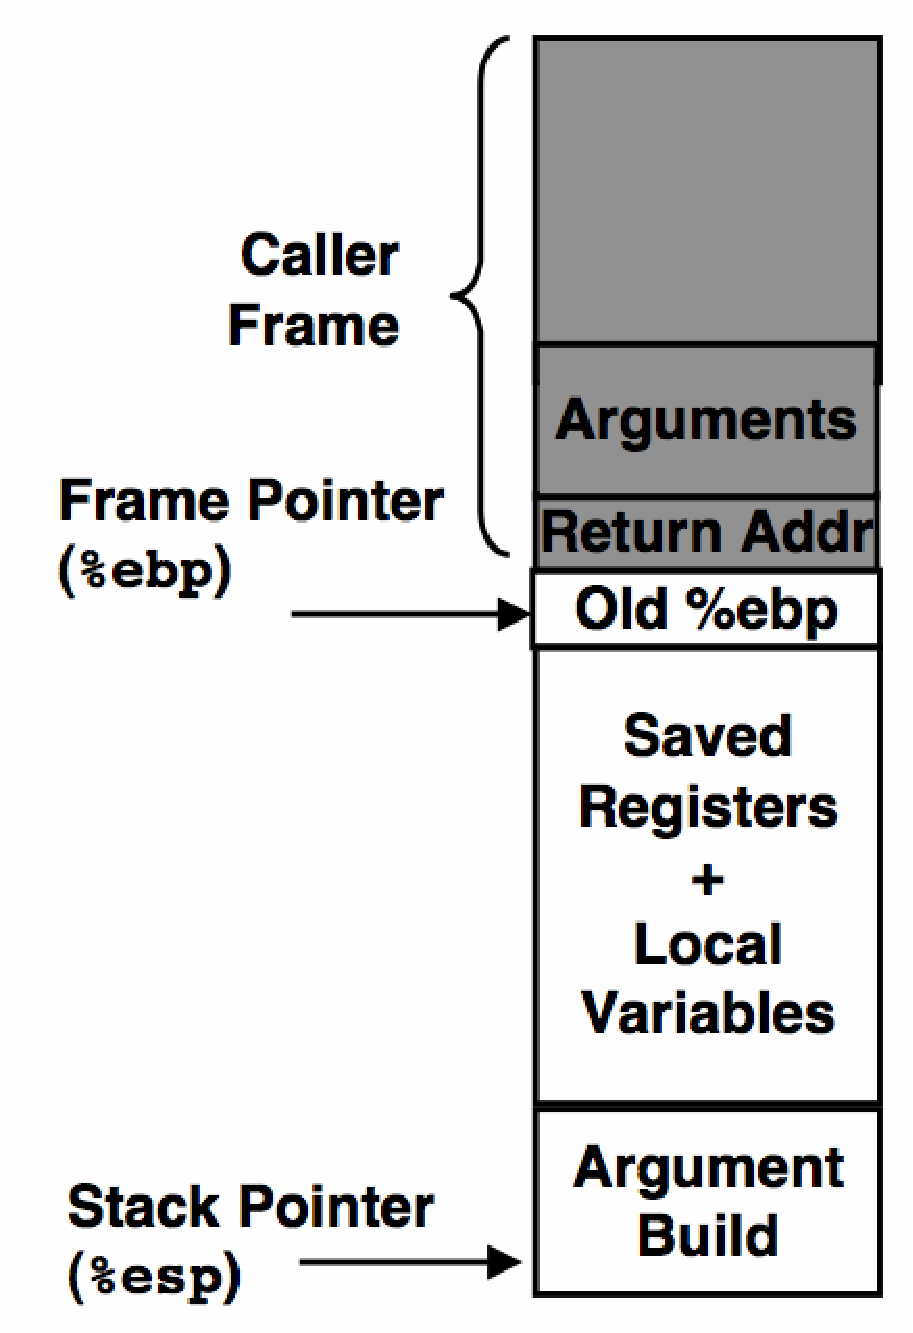
\includegraphics[scale=0.3]{figure/stack}
\caption{栈的结构} \label{fig:stack}
\end{center}
\end{figure}

调试程序很方便的一点,也是非常重要的一点就是停止在断点是可以看到断点所在的调用栈,它告诉你被调试的程序执行到了什么地方,是怎么执行到这里的。
通过对栈的检查,还能看到函数调用时使用的参数,
以及被调用到函数的局部变量等信息。
在~GDB~中,程序的调用栈看起来像这样:
\begin{lstlisting}
(gdb) bt
#0  0x00a1a7a2 in _dl_sysinfo_int80 () from /lib/ld-linux.so.2
#1  0x00c85f7c in pthread_cond_timedwait@@GLIBC_2.3.2 () from /lib/tls/libpthread.so.0
#2  0x0805f271 in ACE_OS::cond_timedwait (this=0x0, abstime=0xb7ffc2a0)
    at /home/cm/ACE_wrappers/ace/OS.i:2772
#3  0x0805f271 in ACE_Condition_Thread_Mutex::wait (this=0x0, abstime=0xb7ffc2a0)
#4  0x0805f271 in ACE_Condition_Thread_Mutex::wait (this=0x0, abstime=0xb7ffc2a0)
#5  0x0804d224 in ACE_Message_Queue<ACE_MT_SYNCH>::wait_not_empty_cond (this=0x80af8b8, mon=...,
    timeout=0xb7ffc2a0) at /home/cm/ACE_wrappers/ace/Message_Queue_T.cpp:1139
#6  0x0804d914 in ACE_Message_Queue<ACE_MT_SYNCH>::dequeue_head (this=0x80af8b8, first_item=@0xb7ffc2bc,
    timeout=0xb7ffc2a0) at /home/cm/ACE_wrappers/ace/Message_Queue_T.cpp:1296
#7  0x0804cf46 in ACE_Task<ACE_MT_SYNCH>::getq (this=0xbffff390, mb=@0xb7ffc2bc, tv=0xb7ffc2a0)
    at /home/cm/ACE_wrappers/ace/Task_T.i:21
#8  0x0804cdfb in cm::TaskManager::svc (this=0xbffff390) at foo.cpp:61
#9  0x0806bf38 in ACE_Task_Base::svc_run (args=0xbffff390) at Task.cpp:203
#10 0x08066d0a in ACE_Thread_Adapter::invoke_i (this=0x80afb38) at Thread_Adapter.cpp:148
#11 0x08066c8a in ACE_Thread_Adapter::invoke (this=0x80afb38) at Thread_Adapter.cpp:91
#12 0x00c833cc in start_thread () from /lib/tls/libpthread.so.0
#13 0x00afd1ae in clone () from /lib/tls/libc.so.6
\end{lstlisting}

检查栈主要使用下面这些命令:

\noindent
\code{backtrace [\param{full}] [\param{n}|\param{-n}]} \index{gdb!backtrace} \index{gdb!bt}

打印出出程序的调用栈。命令缩写为~\code{bt}。
可选参数~\param{full}~表示在打印栈的每一帧时同时打印出该帧上函授调用的参数及函数的局部变量。
可选参数~\param{n}~或~\param{-n}~表示要打印的调用栈的帧数。
如果是正数~\param{n}~表示从栈顶(最后调用的函数)开始计数打印~\param{n}~帧,
如果是负数~\param{-n}~表示从栈底(main函数)开始计数打印~\param{n}~帧。


\subsection{帧(frame)}
因为栈是由帧组成的,所以检查栈上的数据,其实就是和帧打交道。
每一帧包含了函数调用的参数,函数的局部变量以及正在执行的函数的地址。
当程序启动的时候,栈上只有一帧(就是~\code{main}~函数),
通常这一帧称为初始帧(\emph{initial frame})或者最外面的帧(\emph{outermost frame}),
每进行一次函数调用产生新的一帧,当函数调用返回的时候,该帧被销毁。如果函数是递归调用的,会有不停的新的帧产生,如果调用的深度太深,就会导致栈被耗尽。

在程序内部,帧使用帧的地址来标识,
通常会有一个\emph{帧寄存器}用来保存当前帧的指针。

GDB~会对每一帧给以一个编号,最里面的帧(当前正在执行的帧)的编号为~0,
调用它的函数的帧的变化为~1,以此类推\ldots
帧的编号在~GDB~调试中命令会用到。

有些编译器提供了一种优化可以把栈帧优化掉。比如~GCC~提供了优化选项
\code{-fomit-frame-pointer}可以把帧指针优化掉。
GDB~不能很好的处理这类函数调用,因此建议在编译调试版本时不要使用这个优化选项。

和帧相关的命令有下面这些:

\noindent
\code{frame \param{n}}

\paramdesc{切换到第~\param{n}~帧。命令缩写为~\code{f}。
该命令会显示切换到的帧的函数名、参数及指令地址等信息。}


\noindent
\code{up \param{n}}

\paramdesc{向上移动~\param{n}~帧。如果参数缺省:\param{n}=1。
比如当前在第~0~帧的话,\code{up}~之后就移动到第~1~帧了。}

\noindent
\code{down \param{n}}

\paramdesc{向下移动~\param{n}~帧。如果参数缺省:\param{n}=1。
比如当前在第~5~帧的话,\code{up}~之后就移动到第~4~帧了。}

\noindent
\code{info frame [\param{addr}]}

\paramdesc{打印~\param{addr}~所在帧的所有信息,
包括调用帧、参数、局部变量、寄存器等信息。
如果没有指定参数~\param{addr},默认为当前帧。}

\noindent
\code{info args}

\paramdesc{打印当前帧的函数调用的参数。}

\noindent
\code{info locals}

\paramdesc{打印当前帧的局部变量。}

\noindent
\code{info catch}

\paramdesc{打印当前帧的异常捕获句柄。}


示例:
\begin{lstlisting}
(gdb) frame 8
#8  0x0804cdfb in cm::TaskManager::svc (this=0xbffff390) at foo.cpp:61
61	                    if (this->getq(mb, &timeout) < 0) {
(gdb) info args
this = 0xbffff390
(gdb) info frame
Stack level 8, frame at 0xb7ffc320:
 eip = 0x804cdfb in cm::TaskManager::svc (foo.cpp:61); saved eip 0x806bf38
 called by frame at 0xb7ffc360, caller of frame at 0xb7ffc270
 source language c++.
 Arglist at 0xb7ffc318, args: this=0xbffff390
 Locals at 0xb7ffc318, Previous frame's sp is 0xb7ffc320
 Saved registers:
  ebx at 0xb7ffc314, ebp at 0xb7ffc318, eip at 0xb7ffc31c
(gdb) info locals
mb = 0x0
timeout = {...}
workers = {...}
...
\end{lstlisting}


\section{检查源代码}

\subsection{打印源代码}

在~GDB~中使用命令~\code{list}\index{gdb!list}(缩写为~\code{l}~)打印源码,
\code{list}~命令有下面几种格式:

\noindent
\code{list}

\paramdesc{打印当前正在执行的代码。
默认打印源代码的行数为~10~行。
如果重复执行该命令,会连续的打印出紧邻的源代码,
比如上一次~\code{list}~命令打印的源代码行号的范围为213\~222,
那么~\code{list}~命令打印的源代码行号的范围为223\~232。}

\noindent
\code{list [\param{filename}:]\param{lineno}}

\paramdesc{打印指定源文件~\param{filename}~和行号~\param{lineno}~处的代码。
如果没有指定~\param{filename},使用当前正在执行的源代码所在的源文件。}

\noindent
\code{list \param{function}}

\paramdesc{打印指定函数的源代码。}

\noindent
\code{list \param{*address}}

\paramdesc{打印地址~\param{address}~处的源代码。}

\noindent
\code{list -}

\paramdesc{向前打印源代码。
比如上一个~\code{list}~命令打印的源代码行号范围为1138\~1147,
那么~\code{list -}~命令打印的源代码行号范围为1128\~1137。}

\code{list}~命令默认打印的行数为~10~行。
如果要修改打印的行数,需要使用~\code{set listsize}~命令。

\noindent
\code{set listsize \param{count}}

\paramdesc{修改~\code{list}~命令一次打印的源代码的行数。}

\noindent
\code{show listsize}

\paramdesc{显示~\code{list}~命令一次打印的源代码的行数。}

\code{list}~的使用示例:
\begin{lstlisting}
(gdb) list
(gdb) list 1123
(gdb) list foo
\end{lstlisting}

\subsection{编辑源代码}

在调试的时候,发现错误可以立即修改源代码,然后编译之后再继续调试。
GDB~早已经实现这种功能,我们可以使用~\code{edit}~\index{gdb!edit}命令修改源代码。
编辑完成之后执行~\code{make}~命令立即编译,
然后可以在执行~\code{run}~命令重新开始调试。
在重新调试的时候,之前设置的断点依然有效。

\noindent
\code{edit [\param{filename}:]\param{lineno}}

\paramdesc{编辑指定文件~\param{filename}~和指定行号~\param{lineno}~处的源代码。
如果没有指定~\param{filename},使用当前正在执行的代码所在的源代码。}

\noindent
\code{edit \param{function}}

\paramdesc{编辑指定函数~\param{function}~所在的源文件,并定位到该函数。}

\noindent
\code{edit}

\paramdesc{如果不指定参数。编辑当前正在执行的的代码所在的源文件。}

在编辑源代码的时候~GDB~会使用环境变量~\code{EDITOR}~所指定的编辑器作为源代码编辑器。
比如如果你想使用~vim~作为源代码编辑器,需要在执行~\code{gdb}~之前先设置该环境变量。
对于~\code{bash}~的~\code{SHELL},命令为
\begin{lstlisting}
export EDITOR=vim
\end{lstlisting}
对于~\code{csh}~的~\code{SHELL},命令为
\begin{lstlisting}
setenv EDITOR vim
\end{lstlisting}
如果需要保存设置,对于~\code{bash}~的~\code{SHELL},
可以把设置写入~\code{\~/.bash\_profile}。
对于~\code{csh}~的~\code{SHELL},
可以把设置写入~\code{\~/.cshrc}。

\subsection{查找源代码}

在~GDB~中还可以通过关键字字查找源代码,
对应的命令为~\code{search}~和~\code{reverse-search}:
\index{gdb!search} \index{gdb!reverse-search}

\noindent
\code{forward-search \param{regexp}} \\
\code{search \param{regexp}}

\paramdesc{在当前源文件正向查找~\param{regexp},
参数~\param{regexp}~支持正则表达式。命令缩写为~\code{fo}。}


\noindent
\code{reverse-search \param{regexp}}

\paramdesc{在当前源文件反向查找~\param{regexp},
参数~\param{regexp}~支持正则表达式。命令缩写为~\code{rev}。}

示例:
%TODO
\begin{lstlisting}

\end{lstlisting}


\subsection{指定源代码的搜索路径}

在使用~\code{list}~命令的时候,有时候会因为编译的机器和调试的不是同一台的机器的原因,
或者调试时源代码的路径发生了改变,这可能导致~GDB~无法打印源代码。

\noindent
\code{directory \param{dirname} \ldots}

\paramdesc{设置源代码的搜索路径。命令的缩写为~\code{dir}。
针对~UNIX~平台,多个路径名之间使用冒号(:)分隔,
针对~WIN~平台,多个路径名之间使用分号(;)分隔。
使用使用变量~\code{\$cdir}~代表编译目录,
变量~\code{\$cwd}~代表当前工作目录。
}

\noindent
\code{directory}

\paramdesc{重新设置源代码的搜索路径为初始值。
比如在UNIX平台上该值的设置为~\code{\$cdir:\$cwd}。
执行该命令后会提示你确认。}


\noindent
\code{show directories}

\paramdesc{打印源代码的搜索路径。}

示例:
%TODO
\begin{lstlisting}

\end{lstlisting}


\subsection{反汇编}

在~GDB~中可以使用命令~\code{disassemble}~来进行反汇编源代码。

\noindent
\code{disassemble [\param{/m}|\param{/r}] [\param{addr}|\param{func}]}

\paramdesc{从指定的地址~\param{addr}~开始反汇编,
或者反汇编指定的函数~\param{func},
如果没有指定~\param{addr}~和~\param{func},
反汇编当前正在执行的指令。
参数~\param{/m}~指定反汇编的时候同时打印对应的源代码,
参数~\param{/r}~指定反汇编的时候同时打印对应的~16~进制的机器指令。}

示例:
%TODO
\begin{lstlisting}

\end{lstlisting}


\section{检查数据}

调试的时候免不了要打印某个变量的值,数组的值,某个内存地址值等信息。
GDB~提供了丰富的命令来打印这些信息。
GDB~还支持类型之间的强制转换,对数组的操作。

GDB~提供的检查数据的命令有~\code{print}、\code{printf}、\code{x}、\code{output}、
\code{display}~等。

\subsection{打印表达式的值 - \code{print}}

打印某个表达式最常用的命令是~\code{print},缩写为~\code{p}。

\noindent
\code{print [\param{/fmt}] \param{expr}}

\paramdesc{打印表达式~\param{expr}~的值,
可以使用使用参数~\param{fmt}~来进行强制格式转换后再打印,
默认是使用定义的数据类型来打印。
\param{fmt}~支持的格式见表~\ref{tab:print_fmt}。}

\begin{table}[!bhp]
\begin{tabularx}{400pt}{l|X}
\hline
\hline
fmt & 说明 \\
\hline
x & 把~\param{expr}~转换为整数并以~16~进制的格式打印。\\
d & 把~\param{expr}~转换为有符号整数并以~10~进制的格式打印。\\
u & 把~\param{expr}~转换为无符号整数并以~16~进制的格式打印。\\
o & 把~\param{expr}~转换为整数并以~8~进制的格式打印。\\
t & 把~\param{expr}~转换为整数并以~2~进制的格式打印。t代表的含义是two。\\
a & 把~\param{expr}~作为一个地址打印。类似命令~\code{info symbol \param{expr}}。\\
o & 把~\param{expr}~转换为char并打印,如果是不可打印字符,使用'$\backslash$nnn'的格式表示。\\
f & 把~\param{expr}~转换为浮点数并打印。\\
s & 把~\param{expr}~转换为以'$\backslash$0'结尾的字符串并打印。\\
\hline
\hline
\end{tabularx}
\caption{print支持的格式}\label{tab:print_fmt}
\end{table}

\noindent
\code{printf \param{template}, \param{expr}\ldots}

\paramdesc{使用~C~语言的风格的printf来打印表达式~\param{expr}~的值,
多个~\param{expr}~之间使用逗号分隔。}

示例
\begin{lstlisting}
p i
p/x $pc
printf
%TODO
\end{lstlisting}

\subsection{数组}

GDB~支持打印数组,
表达数组在~GDB~中的格式为~\code{\param{array}@\param{len}}。
其中~\param{array}~为数组的名称,\param{len}~为数组的长度。

比如在~C++~中这样定义一个包含3个元素的数组:
\begin{lstlisting}
int* ia = new int[3];
\end{lstlisting}
数组的内容为{111, 222, 333},
我们可以使用~\code{print *ia@3}~来打印数组的内容。
示例如下:

\begin{lstlisting}
(gdb) p ia@3
$4 = {0x87f8018, 0x87f8008, 0xbfe54e78}
(gdb) p *ia@3
$5 = {111, 222, 333}
(gdb) p ia
$6 = (int *) 0x87f8018
(gdb) p *ia
$7 = 111
\end{lstlisting}


\subsection{打印内存中的信息 - \code{x}}

要检查任意内存处的数据,可以使用命令~\code{x}(examine~的缩写)。

\noindent
\code{x\param{/nfu addr}}

\paramdesc{打印内存~\param{addr}~处的数据。
参数~\param{n},\param{f},\param{u}~是可选参数。}

\paramdesc{参数~\param{n}~指定要检查的内存长度,单位由参数~\param{u}~指定。缺省为1。}

\paramdesc{参数~\param{f}~指定打印的格式,参见表~\ref{tab:print_fmt},
另外新增一种格式~\code{i},表示打印汇编指令(instructions)。
缺省为~\code{x}。}

\paramdesc{参数~\param{u}~指定打印的单位。支持的单位见表~\ref{tab:x_param_unit}。
缺省值为~\code{w}。}

\begin{table}
\begin{tabularx}{400pt}{l|X}
\hline
\hline
u & 说明 \\
\hline
b & Bytes.  \\
h & Halfwords (two bytes).  \\
w & Words (four bytes). This is the initial default. \\
g & Giant words (eight bytes). \\
\hline
\hline
\end{tabularx}
\caption{x命令支持的打印单位}\label{tab:x_param_unit}
\end{table}

比如,\code{x/10cb 0x12345}~打印从内存地址~\code{0x12345}~开始处~10(参数\param{n})个~byte(参数\param{b})的字符(参数\param{c})。
\code{x/12xw \$sp}~打印栈指针开始处~12~个字长的~16~进制数。
\code{x/6i \$eip}~打印当前指令接下来的6条指令。使用~\code{x/i \$eip}~可以查看当前正在执行的指令。

示例:
%TODO
\begin{lstlisting}

\end{lstlisting}

\subsection{自动打印某个表达式的值 - \code{display}}

当你要频繁的监视一个表达式的值的时候
(比如在~\code{for}~循环中,打印循环的次数),
使用命令~\code{display}~可以很方便完成这种任务。
\code{display}~会在每次程序中断的时候自动进行打印。

\noindent
\code{display [\param{/fmt}] \param{expr}}

\paramdesc{当程序中断的时候自动打印表达式~\param{expr}~的值。
比如每执行一次~\code{next}~命令,~\param{expr}~的值都会被打印一次。
参数\param{/fmt}~见表~\ref{tab:print_fmt},
另外可以使用~\code{i}~来打印指令。
设置成功后返回一个编号来代表该监视的表达式,
这个编号可以用于删除和禁用该自动监视的表达式。}

\noindent
\code{display}

\paramdesc{打印所有设置了要自动监视的表达式的值。}

\noindent
\code{undisplay \param{dnums} \ldots} \\
\code{delete display \param{dnums} \ldots}

\paramdesc{删除之前使用~\code{display}~设置的要自动监视的表达式。
\param{dnums}~由~\code{display}~命令返回。}

\noindent
\code{disable display \param{dnums} \ldots}

\paramdesc{禁用之前使用~\code{display}~设置的要自动监视的表达式。
\param{dnums}~由~\code{display}~命令返回。}

\noindent
\code{enable display \param{dnums} \ldots}

\paramdesc{启用之前使用~\code{disable}~禁用的自动监视的表达式。
\param{dnums}~由~\code{display}~命令返回。}

\noindent
\code{info display}

\paramdesc{打印所有要自动监视的表达式列表。}

示例:
%TODO

\subsection{打印设置}

GDB~可以控制打印时的一些格式,典型的设置如下:

\noindent
\code{set print pretty \param{on}|\param{off}}

\paramdesc{设置打印~\code{struct/union/class}~的成员时是否分行打印,
设置为~\param{on}~开起来效果要好些,但是如果成员变量很多时就会占用很多行。
效果参见本节的示例。
缺省为~\param{off}。}

\noindent
\code{show print pretty}

\paramdesc{显示~\code{set print pretty}~的设置。}

\noindent
\code{set print object \param{on}|\param{off}}

\paramdesc{}

\noindent
\code{show print object}

\paramdesc{缺省为~\param{on}。}

\noindent
\code{set print vtble \param{on}|\param{off}}

\paramdesc{是否答应C++虚函数表。缺省为~\param{on}。}

\noindent
\code{show print vtble}

\paramdesc{}

\subsection{历史记录}

\code{print}~打印的表达式的值~GDB~都会记录下来,
GDB~在打印的时候会给该表达式指定一个编号~\param{num},
后续在其它的表达式中可以使用~\$\param{num}~来直接引用该表达式的值。

\noindent
\code{show values [\param{n}]}

\paramdesc{打印~GDB~记录的表达式值的历史。
如果指定参数~\param{n},那么最多打印~\param{n}~个历史表达式的值。}

示例:
%TODO

\subsection{内部变量}

\noindent
\code{\$\_}

\paramdesc{}


\noindent
\code{\$\_\_}

\paramdesc{}

\noindent
\code{\$\_exitcode}

\paramdesc{}

\noindent
\code{\$\_siginfo}

\paramdesc{}

\subsection{寄存器}

GDB~中可以打印的寄存器的值,寄存器使用~\$\param{regname},
\param{regname}~是寄存器的名字。
可以使用~\code{info registers}~来打印寄存器信息。

\noindent
\code{info registers}

\paramdesc{打印当前帧除了浮点数和向量寄存器的其它所有寄存器的名字和值。}

\noindent
\code{info all-registers}

\paramdesc{打印当前帧所有寄存器(包括浮点数和向量寄存器)的名字和值。}

示例:
%TODO

\begin{lstlisting}
info registers
p $eax
x/i $eip
\end{lstlisting}

\subsection{如何产生core}

在调试的时候如果想保存正在调试的程序的当前状态以后再来继续分析,
可以通过产生~core~文件来达到此目的。
关于~core~的调试,参考第~\ref{ch:coredump}~章(第~\pageref{ch:coredump}~页)。

\noindent
\code{generate-core-file [\param{file}]}\\
\code{gcore [\param{file}]}

\paramdesc{生成当前正在调试的文件~core~文件,
参数~\param{file}~用于指定~core~文件名,
如果没有指定,默认为~core.\param{pid},
\param{pid}是正在调试的进程的进程号。}

示例:
\begin{lstlisting}
(gdb) gcore
Saved corefile core.6945
(gdb) gcore foo.dump
Saved corefile foo.dump
\end{lstlisting}


\subsection{在内存中查找}

在~GDB~中可以使用~\code{find}~命令在内存中进行搜索。

\noindent
\code{find [\param{/sn}] \param{start\_addr, +len}, \param{val1} [, \param{val2} \ldots]} \\
\code{find [\param{/sn}] \param{start\_addr, end\_addr}, \param{val1} [, \param{val2} \ldots]}

\paramdesc{在指定的内存中查找指定的序列~\param{val1},\param{val2}\ldots
指定的内存要求是连续的,
可以指定开始地址(\param{start\_addr})和长度(\param{len}),
或者指定开始地址(\param{start\_addr})和结束地址(\param{end\_addr})。
\param{s}~和~\param{n}~是可选参数。}

% TODO:

\section{修改执行路径}
在调试时可以通过下面的方法更改程序的执行路径:
\begin{itemize}
\item 修改变量的值
(参见第~\ref{sec:modvar}~节,第~\pageref{sec:modvar}~页);

\item 让函数提前返回并指定想要的返回值
(参见第~\ref{sec:cmd_return}~节,第~\pageref{sec:cmd_return}~页);

\item 给程序发送信号
(参见第~\ref{sec:sendsignal}~节,第~\pageref{sec:sendsignal}~页);

\item 调用指定的函数
(参见第~\ref{sec:cmd_return}~节,第~\pageref{sec:cmd_return}~页);

\end{itemize}

GDB~甚至还能修改你正在调试的二进制文件,俗称patch
(参见第~\ref{sec:makepatch}~节,第~\pageref{sec:makepatch}~页)。

\subsection{修改变量的值}
\label{sec:modvar}

GDB~中可以使用~\code{print}~命令和~\code{set}~来对变量进行赋值。
\code{print}~赋值后之后会打印出新的值,
而~\code{set}~不会打印新的值。
如果不知道要赋值的变量的类型,可以使用~\code{ptype}~来查看。

\noindent
\code{set \param{name} = \param{value}}

\paramdesc{给变量~\param{name}~赋值~\param{value}。}

\noindent
\code{set \{\param{type}\}\param{addr} = \param{value}}

\paramdesc{把内存地址为~\param{addr}存储的数据强制类型转换成~\param{type},
并且赋值为~\param{value}。
示例:\code{set \{int\}0x8aaa01c = 1234}。
}

\noindent
\code{ptype \param{var}}

\paramdesc{打印变量~\param{var}~的类型定义。
比如~\param{var}~是一个class的实例,它会打印该~class~的定义。}

示例:
\begin{lstlisting}
% TODO
p i = 1
set x = 2
set {int}0xddfd = 3
\end{lstlisting}

\subsection{直接跳转}

在调试过程中,可以使用~~命令直接跳转到指定的地址出继续执行。

\noindent
\code{jump \param{lineno}}\\
\code{jump \param{addr}}

\paramdesc{跳转到指定的行号~\param{lineno}~或指定的地址~\param{addr}。
一般预先在掉转的目标地址设置好一次性断点,
在跳转之后就会立即停在这个断点上。
\code{jump}~不会改变当前帧、栈、内存及寄存器的值\footnote{除了指令寄存器PC。},
所以跳转最好在本函数内进行。}

\paramdesc{在某些平台上,可以通过修改寄存器~PC~的值来达到同样的效果。}

\subsection{发送信号}
\label{sec:sendsignal}

在调试的时候,可以向被调试的程序发送信号,使用~\code{signal}~命令。

\noindent
\code{signal \shparam{signo}}

\paramdesc{向被调试的程序发送信号~\param{signo}。
\param{signo}~可以是数字或信号名,
比如~\code{signal 1}~和~\code{signal SIGHUP}~的效果是一样的。}

\paramdesc{如果~\param{signo}~为~0,表示继续执行程序而不处理信号。
在因为信号被中断的情况下,
如果想使程序忽略这个信号继续执行就应该使用“\code{signal 0}”,
而不是~\code{continue},因为~\code{continue}~不会忽略信号。}

\subsection{提前返回}
\label{sec:cmd_return}

在调试的过程可以使用~\code{return}~命令来从当前函数提前返回。

\noindent
\code{return [\param{expression}]}

\paramdesc{不执行当前函数剩下的代码而直接返回。
可选参数~\param{expression}~可以用来指定函数的返回值。
如果你想执行完当前函数然后再返回,应该使用~\code{finish}~命令(第~\pageref{sec:cmd_finish}~页)。}

\subsection{调用函数}

在调试的过程中,可以使用~\code{print}~或~\code{call}~命令调用其它的函数并执行。

\noindent
\code{print \param{func}}\\
\code{call \param{func}}

\paramdesc{执行函数~\param{func}。}

如果函数~\param{func}~执行过程中产生信号,
可以通过~\code{set unwindonsignal}~来控制其行为。
在调用~\code{call}~之前应该先调用~\code{set unwindonsignal}。

\noindent
\code{set unwindonsignal \param{on}|\param{off}}

\paramdesc{如果设置为~\param{on},在~\code{call}~命令执行完之后,
把堆栈恢复到之前的状态。
如果设置为~\param{off},如果在执行~\param{func}~的过程中产生信号,
程序会中断在~\param{func}~中。
缺省为~\param{off}。
}

\code{show unwindonsignal}

\noindent{显示~\code{set unwindonsignal}~的设置。}

\subsection{制作patch}
\label{sec:makepatch}

缺省情况下,GDB~以只读的方式打开被调试的文件和~core~文件。
如果你需要~patch~它们,需要在~GDB~启动的时候指定~\shparam{-write}~参数或者使用~\gdbcmd{set write}~命令。

\noindent
\gdbcmd{set write \gdbcmdparam{on}|\gdbcmdparam{off}}

\paramdesc{设置当前正在调试的二进制文件和~core~文件是否可写。缺省为~\gdbcmdparam{off}。}

\noindent
\gdbcmd{show write}

\paramdesc{显示当前正在调试的可执行文件和~core~文件是否可写。}

示例:
\begin{lstlisting}
$ gdb ./a.out
(gdb) show write
Writing into executable and core files is off.
(gdb) set write on
(gdb) show write
Writing into executable and core files is on.
\end{lstlisting}


\section{GDB的文本界面(TUI)}
\label{sec:tui}
GDB~支持curses的文本窗口模式,称之为TUI - Text User Interface。
TUI能显示如下四个窗口:
GDB在单独的窗口中显示源文件、汇编代码、寄存器信息及GDB的命令输入/输出。

启动TUI的方式是使用~'gdbtui'~或~'gdb -tui'。

\section{自定义GDB命令}

GDB~支持自定义命令,就是说你可以把~GDB~的几个命令组合成新的自定义命令,
而且在自定义的命令中能使用~\gdbcmd{if}~进行条件判断,
使用~\gdbcmd{while}~进行循环等。
自定义命令使用~\gdbcmd{define}~来完成。

\begin{lstlisting}
define cmdname
 ...
 ...
end

document cmdname
  There is help of cmdname.
end
\end{lstlisting}

自定义命令最多可以有~10~个参数,
它们是~\gdbcmdparam{\$arg0}\ldots\gdbcmdparam{\$arg9}。
在命令体中可以使用\gdbcmdparam{\$argc}~来代表传递的参数个数。
\gdbcmd{document}~是可选的,用来定义该自定义命令的帮助信息,
如果定义的话,在~\gdbcmd{help} \gdbcmdparam{cmdname}~的时候会显示该帮助信息。

示例一:需要一个参数的自定义命令:
\begin{lstlisting}
define get_chunk
  if $argc == 1
    set $addr = $arg0
    print (($addr - malloc_start)/4096)*140 + heap_start
  else
    echo Usage: get_chunk addr
  end
end
\end{lstlisting}

在用户自定义的命令中使用~\gdbcmd{if}~的语法如下:
\begin{lstlisting}
if cond
  ...
else
  ...
end
\end{lstlisting}

在用户自定义的命令中使用~\gdbcmd{while}~的语法如下:
\begin{lstlisting}
while cond
  ...
end
\end{lstlisting}

\subsection{定义GDB命令Hook}

在~GDB~中可以定义~GDB~命令的~Hook,即对于~GDB~的命令~\gdbcmd{cmdname},
如果存在自定义的命令~\gdbcmd{foo-cmdname},
那么在执行~\gdbcmd{cmdname}~的时候,会先执行~\gdbcmd{foo-cmdname}。

%TODO: example

\section{GDB初始化文件}

在~GDB~每次启动的时候,都会尝试读取它的初始化文件\$HOME/.gdbinit
并执行。如果想在.gdbinit中执行其它的文件,可以使用source命令。

\noindent
\gdbcmd{source \gdbcmdparam{file}}
\index{gdb!source}

\paramdesc{执行~\gdbcmdparam{file}~中的命令。}


\section{逆向调试(Reverse Debug)}
\index{gdb!逆向调试}

在程序调试时候,你是否有过因为随手的\code{n}就执行一条语句,
之后你才意识意识到你并不想执行\code{n}命令。
一般来说,为了再次遇到这个条件,这就意味这你要重头开始再来调试一次了,
这个时候要是有后悔药就好了,可以回退到之前的状态再来一次,
这样就极大可以加快调试的速度。

\section{GDB的文本界面(TUI)}
GDB~支持curses的文本窗口模式,称之为TUI-Text User Interface。
TUI能显示如下四个窗口:
GDB在单独的窗口中显示源文件、汇编代码、寄存器信息及GDB的命令输入/输出。

启动TUI的方式是使用~'gdbtui'~或~'gdb -tui'。
如果是~GDB~的~shell~下,可以使用组合键~\shcmd{Ctrl-x a}(按住Ctrl同时按x,然后释放Ctrl和x,再按a)来切换到TUI模式。

\subsection{TUI中的组合键}

在~GDB~中支持的组合键如下:

\noindent
\gdbcmd{Ctrl-x a}

\paramdesc{进入或退出TUI模式。}


\noindent
\gdbcmd{Ctrl-x 1}

\paramdesc{只显示~1~个窗口:源代码或汇编窗口。
如果~TUI~没有启动,它会自动启动~TUI。}

\noindent
\gdbcmd{Ctrl-x 2}

\paramdesc{至少打开~2~个窗口。
如果~TUI~没有启动,它会自动启动~TUI。}

\noindent
\gdbcmd{Ctrl-x o}

\paramdesc{改变当前活动的窗口。}

\noindent
\gdbcmd{Ctrl-L}

\paramdesc{刷新当前屏幕。
在调试的时候,如果被调试的平、程序有向屏幕输出的话,
可能会把屏幕弄的很难看,这个时候~\gdbcmd{Ctrl-L}~就派上用场了。}

\subsection{TUI涉及的命令}

\noindent
\gdbcmd{layout next}

\paramdesc{切换到下一个窗口布局模式。
重复该命令,GDB会自动在几种窗口布局中进行切换。
你可以选择你想要的布局模式然后停下来。}

\noindent
\gdbcmd{layout prev}

\paramdesc{切换到上一个窗口布局模式。}

\noindent
\gdbcmd{layout src}

\paramdesc{只显示源代码窗口。}

\noindent
\gdbcmd{layout asm}

\paramdesc{只显示汇编代码窗口。}

\noindent
\gdbcmd{layout split}

\paramdesc{同时显示源代码与汇编代码窗口。}

\section{GDB高级用法}

\subsection{GDB初始化文件}

\subsection{自定义GDB命令}


\section{逆向调试(Reverse Debug)}
\index{gdb!逆向调试}

在程序调试时候,你是否有过因为随手的\code{n}就执行一条语句,
之后你才意识意识到你并不想执行\code{n}命令。
一般来说,为了再次遇到这个条件,这就意味这你要重头开始再来调试一次了,
这个时候要是有后悔药就好了,可以回退到之前的状态再来一次,
这样就极大可以加快调试的速度。
在不确定程序bug的时候,使用逆向调试也是很有帮助的,
可以在可能产生错误的地方反复调试,最终找到bug的根源。

在GDB 7.0的版本开始支持\emph{逆向调试}。
\emph{逆向调试}当前仅在有限的平台上支持,
\code{i386}和\code{amd64}是支持\emph{逆向调试}的。

\emph{逆向调试}中用到的命令:

\noindent
\code{reverse-continue}(缩写为'rc')

Continue program being debugged but run it in reverse

\noindent
\code{reverse-finish}

Execute backward until just before the selected stack frame is called

\noindent
\code{reverse-next} ('rn')

Step program backward, proceeding through subroutine calls.

\noindent
\code{reverse-nexti} ('rni')

Step backward one instruction, but proceed through called subroutines.


\noindent
\code{reverse-step} ('rs')

Step program backward until it reaches the beginning of a previous source line

\noindent
\code{reverse-stepi}

Step backward exactly one instruction

\noindent
\code{set exec-direction [\param{forward}|\param{reverse}]}

Set direction of execution.

All subsequent execution commands (continue, step, until etc.) will run the program being debugged in the selected direction.

Breakpoints and watchpoints will work in reverse -- allowing you for instance to proceed directly to the previous point at which a variable was modified.


https://sourceware.org/gdb/wiki/ReverseDebug



\section{使用GDB查看STL容器}
\index{gdb!查看STL容器}

如果是用~GDB~的\emph{print}命令来打印~STL~容器(如~vector,stack,set~等),
得到的结果是很难读。

\subsection{GDB 7.0}
GDB7.0能通过Python的pretty-printers\index{gdb!pretty-printers}支持更友好的打印STL容器的信息。

设置步骤如下:

1. 获取~Python libstdc++~的printers:
\begin{lstlisting}[language={sh}]
mkdir -p ~/.gdb/gdb_printers
cd ~/.gdb/gdb_printers
svn co svn://gcc.gnu.org/svn/gcc/trunk/libstdc++-v3/python
\end{lstlisting}

2. 修改\emph{\$HOME/.gdbinit},添加如下几行:
\begin{lstlisting}
python
import sys
sys.path.insert(0, '/home/maude/gdb_printers/python')
from libstdcxx.v6.printers import register_libstdcxx_printers
register_libstdcxx_printers (None)
end
\end{lstlisting}

\subsection{GDB 6.x}
现实是现在Linux发行版中很少有使用~GDB 7.0~的。但是通过~GDB~的自定义命令,
可以很方便的查看STL容器的内容。Dan Marinescu已经写了这样一个GDB的宏包,
当前版本是1.0.3,文件名是stl-view-1.0.3.gdb。

使用方法:
把stl-view-1.0.3.gdb放在\emph{\$HOME/.gdb/}下。
在\emph{\$HOME/.gdbinit}中加入如下一行:
\begin{lstlisting}
source ~/.gdb/stl-view-1.0.3.gdb
\end{lstlisting}

然后可以使用下表的命令来打印STL容器的内容
\index{gdb!pvector} \index{gdb!plist} \index{gdb!pmap} \index{gdb!pset}
\index{gdb!pdequeue} \index{gdb!pstack}
\begin{table}[!bhp]
\begin{tabular}{l|l}
\hline
\hline
容器类型 & GDB命令      \\
\hline
std::vector<T>          &       pvector stl\_variable    \\
std::list<T>	        &       plist stl\_variable T    \\
std::map<T,T>	        &       pmap stl\_variable       \\
std::multimap<T,T>      &       pmap stl\_variable       \\
std::set<T>	        &       pset stl\_variable T     \\
std::multiset<T>        &       pset stl\_variable       \\
std::deque<T>	        &       pdequeue stl\_variable   \\
std::stack<T>	        &       pstack stl\_variable     \\
std::queue<T>	        &       pqueue stl\_variable     \\
std::priority\_queue<T>	&       ppqueue stl\_variable    \\
std::bitset<n>td>	&       pbitset stl\_variable    \\
std::string	        &       pstring stl\_variable    \\
std::widestring	        &       pwstring stl\_variable   \\
\hline
\hline
\end{tabular}
\caption{打印STL容器的GDB命令列表}
\end{table}

\subsection{使用示例}
std::vector<int> iv;
在gdb中使用pvector来打印出iv的内容:\\
(gdb) pvector iv;

%TODO: 范例

更多的信息参考:
https://sourceware.org/gdb/wiki/STLSupport\cite{gdb-stl-support}

\section{GDB的图像界面DDD}
\index{DDD}

\section{F.A.Q}

\begin{enumerate}
\item \textbf{Q}:在~GDB~的输出有很多行时会提示
“Type <return> to continue, or q <return> to quit“,
如何取消这个限制,让~GDB~一次性完成输出?

\textbf{A}:使用\code{set height 0}或者\code{set pagination off}。

\item \textbf{Q}:在~\code{print}~命令中类型强制转换:
\code{p *(cm::Foo*)0x85cf008},
提示“A syntax error in expression, near `)0x85cf008'”,
如何解决?

\textbf{A}:这是因为”\code{::}“的原因,
需要使用单引号把要要转换的类型引起来,
像这样:\code{p *('cm::Foo'*)0x85cf008}~就可以了。

\item \textbf{Q}:如何调试C++的异常?

\textbf{A}:\emph{方法一}:可以使用~GDB~的~\code{catch throw}~在catch上设置\emph{catchpoint}
(参见第~\ref{sec:gdb_catchpoint}~节,第~\pageref{sec:gdb_catchpoint}~页)。

\emph{方法二}:如果程序是使用~GCC~编译器编译的话,
可以在函数~\code{\_Unwind\_RaiseException}~上设置断点。
效果和\emph{方法一}类似。

\emph{方法三}:如果你已经知道要\code{throw}的名称,
而且这个异常是你自己定义的异常,
那么你还可以在你的异常类的构造函数上设置断点。

\item \textbf{Q}:我的~GDB~版本是~6.3,我想在上面调试~C++~异常,
可是~\code{catch throw}~返回错误:
“Function "\_\_cxa\_throw" not defined”,我该怎么办?

\textbf{A}:升级到GDB 7.0。

\item \textbf{Q}:使用~GDB~检查~core~文件时候提示:
“BFD: Warning: foo-15591.core is truncated: expected core file size >= 616845312, found: 314601472.”,这是怎么回事?
\begin{lstlisting}
(gdb) bt
#0  0x082fb2d8 in std::list<xmlnode*, std::allocator<xmlnode*> >::empty (this=Cannot access memory at address 0xb6b70160)
    at /usr/lib/gcc/i386-redhat-linux/3.4.6/../../../../include/c++/3.4.6/bits/stl_list.h:671
Cannot access memory at address 0xb6b7015c
\end{lstlisting}

\textbf{A}:core~文件被截断了。可能的原因有:

\emph{原因一}:产生~core~的时候磁盘没有空间了?

\emph{原因二}:系统设置了~core~文件的大小限制,
对于是~\code{bash}~的~\code{SHELL},使用命令“\code{ulimit -c}”检查,
如果设置了限制,使用命令“\code{ulimit -c unlimited}”取消限制。
如果~\code{csh}的~\code{SHELL}~对应的命令为~\code{limit}。


\item \textbf{Q}:

\textbf{A}:

\end{enumerate}



\section{总结}

关于GDB的更多信息参见GDB在线手册\cite{gdb-man}。

关于GDB的书籍有:

Debugging with GDB: The GNU Source-Level Debugger\cite{debugging-with-gdb}。
在网上能找到这本书的电子版。本章的大部分内容来自该书。

GDB Pocket Reference\cite{gdb-pocket-ref}。

GDB~的在线文档:
https://sourceware.org/gdb/download/onlinedocs/
